\section{Marco Teórico}

    
    
    \subsection{Redes Neuronales Artificiales}

        
        Las redes neuronales artificiales (RNA) son procesos los cuales contienen simples unidades de procesamientos. \\
        Como se puede observar, al mencionar RNA lo primero que se viene a la mente es el procesamiento biol\'ogico por el que transita el 
        cerebro humano. El m\'etodo principal de las redes neuronales es sacarle el máximo poder a los algoritmos de aprendizaje maquina, ya que las redes neuronales 
        tienes un antecedente biol\'ogico.

        Presentan demasiadas utilidades las cuales ayudan a  resolver problemas como los siguientes \cite{liu2015}: 
        no linealidad, mapeo entrada-salida, aprendizaje robusto a errores en los datos de entrenamiento, entre otros.

        Existen varios tipos de Redes Neuronales tales como: Redes Neuronales de Perceptr\'on Multicapa, Redes Neuronales Convolucionales, entre otras.
    
        \subsection{Redes Neuronales de Perceptr\'on Multicapa}

(REVISAR REDACCIÓN Y MEJORARLA)
            Mapear el progreso de una red sirve para conocer y buscar un camino adecuado entre la capa de entrada y salida, esto se puede hacer 
            con problemas de una sola neurona, no obstante, los problemas no lineales no se pueden resolver, para ello se usan los perceptrones
            multicapas, los cuales rompen con esta limitaci\'on.

            Estas neuronas est\'an compuestas de 3 capas como se muestra en la Figura \ref{fig:fig1}.
            Los datos de entrada se van a ir propagando capa por capa, hasta llegar a la capa final, donde la información pasará
            por una funci\'on de activaci\'on la cual permite tener en un rango controlado los valores que se propagan por la red. Al final, las neuronas de la capa de salida darán el resultado esperado o muy próximo a él, si el valor no es correcto, se deberá proceder a una etapa de entrenamiento \cite{liu2015}.

            \begin{figure}[H]
                \centering
                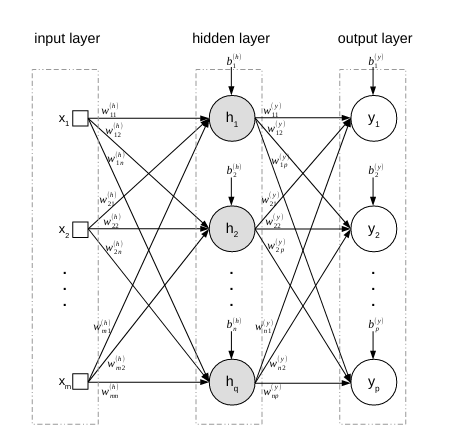
\includegraphics[width=\columnwidth]{MLP.png}
                \caption{Red Neuronal de Perceptr\'on Multicapa \cite{liu2015}}
                \label{fig:fig1}
            \end{figure}


\subsection{Algoritmo Backpropagation}
(Aquí describan este algoritmo, la página que les pase de John les puede ayudar. Términos importantes de escribirlo porque sobre él se basaron para hacer la implementación de las redes con pesos duplicados)


        \subsection{Redes Neuronales Convolucionales}

            Este tipo de red trabaja con el uso de imágenes, por lo general de alta calidad, el \'unico problema que se tiene 
            al momento de que sean de alta resoluciones son que el tiempo de entrenamiento sea enorme y el tiempo de testo (Tengo duda de que la palabra testo quede, puedes checarlo? si no pues dejalo asi jsjs)sea muy tardío.

            Consta de diversas multicapas alternadas, al final tiene una red perceptr\'on multicapa. (REVISEN LA REDACCIÓN, ESTÁ MUY SEGMENTADA LAS IDEAS, TIENEN QUE EXPLICAR UN POCO MÁS PARA QUE SE ENTIENDA MEJOR, TOMEN COMO BASE LA REDACCIÓN QUE LES PONGO AL INICIO DEL TRABAJO, VEAN CÓMO VOY A EXPLICANDO MÁS COSAS, Y AUNQUE ME LLEVO MÁS ESPACIO, QUEDA MEJOR)
            La entrada de una red convolucional, con diferentes medidas en altura y anchura de imagen, para el uso 
            de los proyectos se trabajan en escalas de grises, las cuales contienen filtros y cada filtro tiene distintos 
            rasgos y características de tamaño. Cada capa es submuestreo de m\'inimo a m\'aximo, muestra donde se toman valores 
            desde 2 im\'agenes pequeñas hasta no mas de 5 im\'agenes grandes.

            Antes o despu\'es del submuestreo se aplica la activaci\'on sigmoidal para cada mapeo de rasgos \cite{duran2017}.

            \begin{figure}[H]
                \centering
                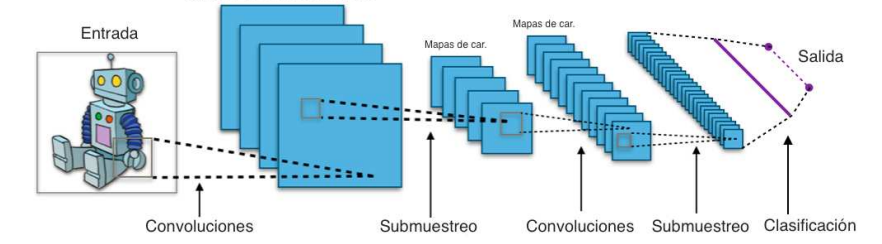
\includegraphics[width=\columnwidth]{esquemaRedConvolucional.png}
                \caption{Esquema de una Red Convolucional \cite{duran2017}}
                \label{fig:fig2}
            \end{figure}

Así como las redes convolucionales, también existen las redes profundas(deep learning), sin embargo, como se comenta en esta sección \label{sec:delimitation} el presente trabajo solo se basará en redes del tipo multicapa perceptron usando el algoritmo de bacpkpropagation, donde de ser demostrados los principios descritos, se podrá aplicar a cualquier otro tipo de algoritmo de aprendizaje.  (LUIS Y SANDRA, AGREGUEN A LA DELIMITACIÓN LO QUE ESTOY INDICANDO AQUÍ, PARA QUE TENGA SENTIDO ESTO)



\subsection{Aprendizaje}

\subsubsection{Aprendizaje en humanos}
        El humano tiene una forma de aprendizaje muy particular, la cual se basa del estudio, donde lee, escribe y practica acerca de
        su tema de interés, pero dicho aprendizaje se puede ir olvidando, esta es una acción muy común que a cualquier persona le sucede.
        Existen estudios donde se comenta que existen tres motivos del porque se olvidan las cosas, proviene parte de la regularización de las emociones,
        el como se adquirieron los conocimientos, y porque el olvido es un proceso por el cual el ser humano transita a lo largo de su vida \cite{Nrby2015}. Pero cabe
        mencionar que esto no es lo único que causa la perdida de memoria, ya que existe la déficit de memoria. 

    \subsubsection{Aprendizaje Humano}
        Al momento de hablar del aprendizaje humano, se debe de hablar de la ciencia cognitiva, que es quien se encarga de descubrir esta incógnita,
        esta ciencia lo estudia de un modo multidisciplinario, el cual abarca las \'areas de \cite{bransford2000}: antropología, lingüística, 
        filosofía, sicología del desarrollo, ciencia de la computación, neurociencia.
        Con el método de esta ciencia se pueden descubrir dos tipos de aprendizaje que son: el aprendizaje con compresi\'on y el aprendizaje Activo.
        
        \subsubsection{Aprendizaje con Compresi\'on}
            La comprensi\'on es una actividad la cual se ha generado al momento de realizar cualquier tipo de lectura.\\
            Teniendo un enfocamiento en el \'ambito estudiantil, ya que es donde m\'as se maneja esta t\'actica, esto es una
            practica algo compleja, sistemática y organizada, pues da el significado de la literatura, gracias a esto se puede
            obtener el contexto de la literatura.
            (Insisto que lo anterior esta mal dicho, pero no se me ocurre de que manera expresarlo)

            Al conocer esto se puede decir con seguridad que para cualquier tipo de aprendizaje la comprensi\'on es 
            una parte primordial \cite{perez2014}.
            (Tambien siento que se debe de agregar un concepto en si o como dice Landassuri mas explicado)

        \subsubsection{Aprendizaje Activo}
            El aprendizaje de la forma en la que se conoce no es del todo efectiva, ya que el sistema educativo
            no se basa en el principio de \textit{belongingness}, el cual esta asociado al estimulo con su respuesta,
            y esto es lo m\'as importante para que el ser humano pueda aprender cualquier cosa.\\
            Este tipo de aprendizaje se basa en la recepci\'on de conocimientos y la pr\'actica donde se ponen en marcha los conocimientos adquiridos.\\
            Otro concepto importante aqu\'i es la tautolog\'ia doble (\textit{selbstt\"atiges Lernen}), que en palabras informales es convertirse en autodidacta, 
            se puede observar que esto pertenece a dicho aprendizaje, porque usa el principio mencionado anteriormente \cite{Huber2008}.
   

 \subsubsection{Aprendizaje Incremental}
        Con el pasar de los años la tecnología a evolucionado, eso quiere decir que el Aprendizaje Automático se ha actualizado y que la 
        cantidad de datos va aumentado con más frecuencia.
        
        Se puede verificar como \textit{"Una tarea de aprendizaje es incremental si los ejemplos de entrenamiento usados para 
        resolverla están disponibles en horas extras, generalmente uno a la vez"} \cite{GiraudCarrier2000}, si los resultados no se 
        necesitan de manera urgente, este tipo de trabajos serán resueltos por algoritmos de aprendizaje no incremental. 

        Una área donde esto es de mucha utilidad es la \textit{Rob\'otica} porque este necesita estar en constante entrenamiento \cite{GiraudCarrier2000}.

        Dicha forma de aprender fue inspirada en la forma en que el humano aprende y esta más rápida, fue por esto que fue adoptada 
        por el aprendizaje m\'aquina.

        Con el paso del tiempo se ha convertido en un paradigma del aprendizaje automático, aquí el aprendizaje toma el lugar de nuevos ejemplos para juntarlos 
        y conforme van aprendiendo estos toman el lugar de los ejemplos ya aprendidos \cite{liu2015}.

        \subsubsection{Algoritmos de Aprendizaje Incremental}
            \textit{"Un algoritmo de aprendizaje es incremental si,
            para cualquier muestra de entrenamiento dada:
            \begin{equation}
                e_{1} , .... , e_{s}
			\end{equation}
            produce un secuencia de hipótesis 
            \begin{equation}
                h_{0} , h_{1}, . . . , h_{n} 
            \end{equation}
            tal que hi+1 depende solo de hola(Tengo duda con la palabra hola si lo tradujiste fijate bien que hayas copiado bien, luego los simbolos no los copia como es ) y del ejemplo actual e"} \cite{GiraudCarrier2000}, como se 
            observa, estos son algoritmos que permiten a la inteligencia artificial poder realizar actividades de predicci\'on 
            de una manera m\'as eficaz.\\
            Un ejemplo del uso de esta rama es el proyecto \textit{COBWEB}, donde se trata de categorizar el n\'umero de Cl\'uster y la pertenencia 
            de dichas categor\'ias por medio de una m\'etrica probabil\'istica global, esto lo realiza por medio de que se agrega 
            una nueva categor\'ia, este proceso lo que realizar\'a es actualizar todas las probabilisticas con los nuevos datos recabados \cite{fisher1987}.


AQUÍ FALTA DESCRIBIR A DETALLE CÓMO SE LLEVA ACABO EL APRENDIZAJE INCREMENTAL, SE PUEDEN BASAR EN EL TRABAJO DE BULLINARIA Y LEANR ++, EXPLIQUENLO A DETALLE PARA QUE SEA SU ESTADO DEL ARTE

